% This is a self-contained tex taken from USENIX style latex template. 
\documentclass[letter,twocolumn,10pt]{article}
\usepackage[margin=1in]{geometry}
\usepackage{enumitem}
\usepackage{url}
\usepackage{makecell}
\usepackage{csquotes}
\usepackage{booktabs}
\usepackage{tabularx}
\usepackage{tikz}
\usepackage{amsmath}
\usepackage{graphicx}
\usepackage{subfig}
\usepackage{float}
\usepackage{caption}
%\usepackage{subcaption}
\usepackage[numbers,sort&compress]{natbib}
\usepackage[super]{nth}
\usepackage{breakurl}
\usepackage[breaklinks]{hyperref}
\def\UrlBreaks{\do\/\do-}

\setlength{\textheight}{9.0in}
\setlength{\columnsep}{0.33in}
\setlength{\textwidth}{7.00in}
\setlength{\topmargin}{0.0in}
\setlength{\headheight}{0.0in}
\setlength{\headsep}{0.0in}
\addtolength{\oddsidemargin}{-0.25in}
\addtolength{\evensidemargin}{-0.25in}

\def\@maketitle{\newpage
 \vbox to 2.5in{
 \vspace*{\fill}
 \vskip 2em
 \begin{center}%
  {\Large\bf \@title \par}%
  \vskip 0.375in minus 0.300in
  {\large\it
   \lineskip .5em
   \begin{tabular}[t]{c}\@author
   \end{tabular}\par}%
 \end{center}%
 \par
 \vspace*{\fill}
 }
}

\usepackage{listings}
\usepackage{xcolor}
\definecolor{codegreen}{rgb}{0,0.6,0}
\definecolor{codegray}{rgb}{0.5,0.5,0.5}
\definecolor{codepurple}{rgb}{0.58,0,0.82}
\definecolor{backcolour}{rgb}{0.95,0.95,0.92}
\lstdefinestyle{mystyle}{
    backgroundcolor=\color{backcolour},   
    commentstyle=\color{codegreen},
    keywordstyle=\color{magenta},
    numberstyle=\tiny\color{codegray},
    stringstyle=\color{codepurple},
    basicstyle=\ttfamily\footnotesize,
    breakatwhitespace=false,         
    breaklines=true,                 
    captionpos=b,                    
    keepspaces=true,                 
    numbers=left,                    
    numbersep=5pt,                  
    showspaces=false,                
    showstringspaces=false,
    showtabs=false,                  
    tabsize=2
}
\lstset{style=mystyle}

\begin{filecontents}{\jobname.bib}
@Book{arpaciDusseau18:osbook,
  author =       {Arpaci-Dusseau, Remzi H. and Arpaci-Dusseau Andrea C.},
  title =        {Operating Systems: Three Easy Pieces},
  publisher =    {Arpaci-Dusseau Books, LLC},
  year =         2015,
  edition =      {1.00},
  note =         {\url{http://pages.cs.wisc.edu/~remzi/OSTEP/}}
}
@InProceedings{waldspurger02,
  author =       {Waldspurger, Carl A.},
  title =        {Memory resource management in {VMware ESX} server},
  booktitle =    {USENIX Symposium on Operating System Design and
                  Implementation (OSDI)},
  year =         2002,
  pages =        {181--194},
  note =         {\url{https://www.usenix.org/legacy/event/osdi02/tech/waldspurger/waldspurger.pdf}}
}
@inproceedings{CooperSTRS10socc,
  author    = {Brian F. Cooper and
               Adam Silberstein and
               Erwin Tam and
               Raghu Ramakrishnan and
               Russell Sears},
  title     = {Benchmarking cloud serving systems with {YCSB}},
  booktitle = {Proceedings of the 1st {ACM} Symposium on Cloud Computing, SoCC 2010,
               Indianapolis, Indiana, USA, June 10-11, 2010},
  pages     = {143--154},
  year      = {2010},
  doi       = {10.1145/1807128.1807152}
}
@misc{leveldb,
    author={Google},
    title={LevelDB},
    howpublished={\url{https://github.com/google/leveldb}}
}
@misc{rocksdb,
    author={Facebook},
    title={RocksDB},
    howpublished={\url{https://github.com/facebook/rocksdb}}
}
@inproceedings{usenixsilk,
author = {Oana Balmau and Florin Dinu and Willy Zwaenepoel and Karan Gupta and Ravishankar Chandhiramoorthi and Diego Didona},
title = {{SILK}: Preventing Latency Spikes in Log-Structured Merge Key-Value Stores},
booktitle = {2019 {USENIX} Annual Technical Conference ({USENIX} {ATC} 19)},
year = {2019},
isbn = {978-1-939133-03-8},
address = {Renton, WA},
pages = {753--766},
url = {https://www.usenix.org/conference/atc19/presentation/balmau},
publisher = {{USENIX} Association},
month = jul,
}

\end{filecontents}

\begin{document}

\date{}

%-------------------------------------------------------------------------------
%TODO You should come up with a compelling title. 
\title{\Large \textbf{A Dynamic Approach to Tune LevelDB’s Hyperparameters for Better Write Performance}}
%TODO Your name. 
\author{Kai Li, Qi Zhang and Yili Luo}
%-------------------------------------------------------------------------------
\maketitle

%-------------------------------------------------------------------------------
\section*{Abstract}
%-------------------------------------------------------------------------------
Existing implementations of LSM key-value stores (e.g., LevelDB, RocksDB) incur high tail latency due to the interference between clients’ operations and LSM internal operations, namely the compactions. In this project, we aim to solve this problem by introducing a dynamic approach to tune the hyper-parameters related to the compaction work in LSM. At the high level, our approach increases the hyper-parameters when facing write-intensive workloads (correspondingly allows much more SSTable files at level 0) and decreases the hyper-parameters when facing read-intensive workloads (correspondingly allows much less SSTable files at level 0). Specifically, we built a workload monitor to collect the most recent clients’ operations, by calculating the read-to-write ratio, the workload monitor is able to indicate the current workload’s feature. To dynamically tune the hyper-parameters, we leverage feedback-control algorithms such as AIMD and MIMD. We implemented our approach atop LevelDB. Compared with native LevelDB, our implementation, LevelDBSILK demonstrated improved write performance without degrading the read performance.
%-------------------------------------------------------------------------------
\section{Introduction}
%-------------------------------------------------------------------------------
Log-Structured-Merge (LSM) tree is designed to improve the performance when processing write-intensive workloads. The most two popular implementations of LSM key-value store are LevelDB ~\cite{leveldb} and RocksDB ~\cite{rocksdb}. However, current implementations incur high tail latency when handling write-intensive workloads. The root cause comes from the interference between clients' operations (reads/writes) and LSM internal operations (e.g., compactions). The internal operations may use up the system's IO bandwidth and thus block the flushing work of memtable and evetually lead to a full memtable which blocks the clients' write operations. To mitigate this problem, we propose a novel technology which dynamically tunes the Hyperparameters related to the compactions. We identified 2 Hyperparameters in LevelDB which control the number of SSTable files at level 0, our approach \textbf{LevelDBSILK} works by increasing these Hyperparameters (which correspondingly allows more files at level 0) when facing write-intensive workloads and decreasing them (allow much less files at level 0) when facing read-intensive workloads. Specifically, we built a workload monitor to track the most recent clients’ operations, including both read and write operations. By calculating the read-to-write ratio, the workload monitor is able to tell the current workload’s feature whether it is read-intensive or write-intensive. Once we obtained the current workload's feature, we feed the feature into the Hyperparameters adjustment component to tune the Hyperparameters accordingly. In the Hyperparameters adjustment component, we implemented both Additive Increase Multiplicative Decrease (AIMD) and Multiplicative Increase Multiplicative Decrease (MIMD) algorithms. We implemented our approach on top of LevelDB and evaluated it by runing different workloads specified in \textsf{db\_bench}. The evaluation results show that compared with the native LevelDB, our approach LevelDBSILK can improves the write performance by $3X$ without degrading the read performance.

The remainder of this report are orginized as follows. In section ~\ref{sec:preliminary}, we introduce the preliminaries of our project. Section ~\ref{sec:implementaion} elaborates on our implementation of SILK in LevelDB. Section ~\ref{sec:evaluation} evaluates the LevelDBSILK and compares it with LevelDB. Section ~\ref{sec:conclusion} concludes the report.
%-------------------------------------------------------------------------------
\section{Preliminaries}
\label{sec:preliminary}
This section provides some preliminaries of this project.

\subsection {LevelDB's Compaction}
\label{sec:leveldbcom}
To implement SILK in LevelDB, the first step is to understand how LevelDB conducts the compaction work. LevelDB adopts two levels of compactions, namely minor compaction and major compaction. Figure ~\ref{leveldb_comaction} shows the Function Call Graph (FCG) of compaction in LevelDB. We elaborate on these two compactions as follows.

\begin{figure*}[!htbp]
\centering
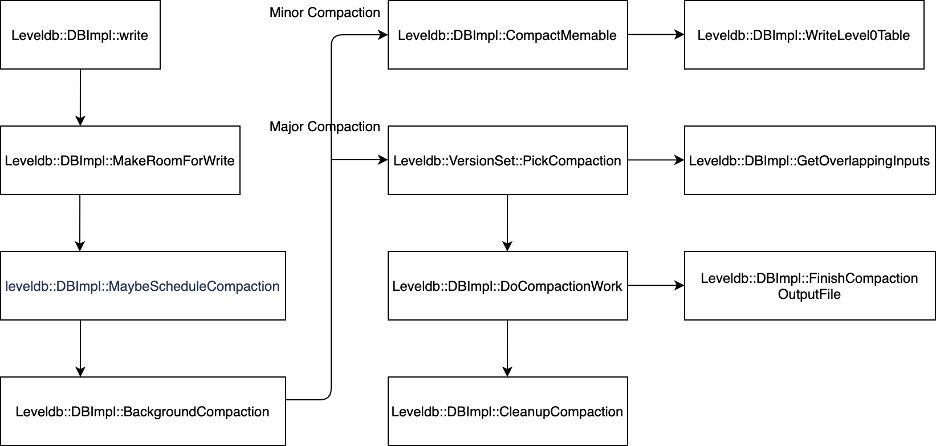
\includegraphics[width=0.8\textwidth]{./leveldb_comaction.png}
\caption{Compaction Function Call Graph in LevelDB}
\label{leveldb_comaction}
\end{figure*}

LevelDB adopts a single thread to do compaction. Once a write operation starts, it will call the \textit{Write} function, inside \textit{Write}, \textit{MakeRoomForWrite} will be triggered. \textit{MakeRoomForWrite} implements a write control mechanism using two Hyperparameters: \textit{kL0\_SlowdownWritesTrigger} (8 by default) and \textit{kL0\_StopWritesTrigger} (12 by default). If the number of files at level 0 reaches to \textit{kL0\_SlowdownWritesTrigger}, LevelDB will slow down each write operation by 1ms. If the number of file reaches to \textit{kL0\_StopWritesTrigge}, all writes will be blocked. 

\textit{MaybeScheduleCompaction} is the entry of the actual compaction work. Three conditions can trigger this function to be executed.
\begin{enumerate}
\item \textit{manual\_compaction\_ != NULL}, user triggers the compaction manually.
\item \textit{imm\_ != NULL}, the Memtable is not NULL pointer and needs to be dumped to SSTable. This refers to the minor compaction.
\item \textit{versions\_$-$$>$NeedsCompaction}, some level needs compaction according to the compaction score. This refers to the major compaction.
\end{enumerate}

Then the thread will continue to invoke \textit{BacgroundCompaction} and start minor compaction and major compaction based on the above conditions.
For a minor compaction, it will be triggered as long as the following two conditions hold simutaneously: 1) memtable exceeds 4MB (defined by \textit{options\_.write\_buffer\_size}); 2) \textit{immutable == NULL}, the Memtable will be rotated to an immutable Memtable first which is further dumped to an SSTable and inserted to the disk.
 
For a major compaction, it will be triggered by one of following four conditions: 1) Manual trigger; 2) \textit{allowed\_seek} used up, every file has a seek limitation, once a seek miss happens, this number will be decreased by one and once it s used up, the compaction will start; 3) The numner of files at level 0 exceeds \textit{kL0\_CompactionTrigger} (4 by default); 4) Size at level i (i$>$0) exceeds $10^i$ MB.

\begin{figure*}[!htbp]
\centering
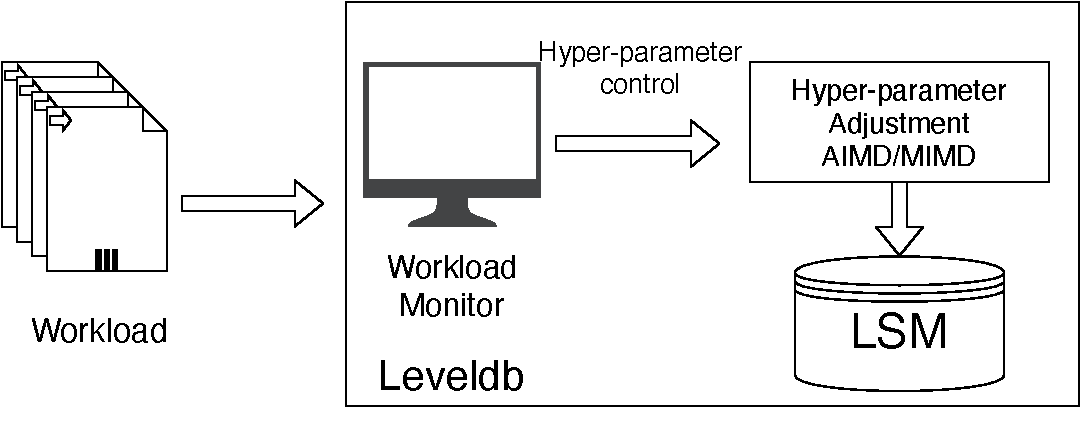
\includegraphics[width=0.8\textwidth]{./system.pdf}
\caption{LevelDBSILK System}
\label{system}
\end{figure*}

\subsection{Feedback Control}
A Feedback Control System is a system which tends to maintain a prescribed relationship of one system variable to another by comparing functions of these variables and using the difference as a means of control.  The Feedback control template for the network congestion is defined as:
$$ w(t+1) = \begin{cases} a_I+b_I*w(t)  & \quad \text{\scriptsize{congestion not detected, Increase}}
 \\a_D + b_D*w(t) & \quad \text{\scriptsize{congestion detected, Decrease}} \end{cases} $$
From the template, we can see there are multiple combinations of feedback control methods with parameters a and b. Based on the existing consequence~\cite{tcp:congestion:control}, only additive-increase/multiplicative-decrease (AIMD) and multiplicative-increase/multiplicative-decrease (MIMD) can achieve efficiency.
Therefore, we only consider these two algorithms in our dynamic tuning approach. 

\subsubsection{AIMD}
The Mathematical Formula for AIMD~\cite{wiki:aimd} is defined as follows:
$$ w(t+1) = \begin{cases}  w(t)+a    & \quad a>1
\\ w(t)*b & \quad 0<b<1 \end{cases} $$
b is typically 0.5. 

\subsubsection{MIMD}
The Mathematical Formula for MIMD is defined as follows:
$$ w(t+1) = \begin{cases}  w(t)*b_I    & \quad b_I>1
 \\w(t)*b_D & \quad 0<b_D<1 \end{cases} $$
In the later section, we will implement these two feedback-control algorithms and compare their performance.

%-------------------------------------------------------------------------------
\section{Implementation}
\begin{table*}[ht]
	\centering 
	%\footnotesize
        %\begin{tabularx}{.8\textwidth}{lXXr}
	\begin{tabular}{c|l|c|c}
		\hline
		\bf{{Workloads}} & \bf{{LevelDB}}  & \bf{{LevelDBSILK (AIMD)}} & \bf{{LevelDBSILK (MIMD)}}\\ \hline
		fillseq & \makecell{6.657 ms} & 6.681 ms & 6.626 ms \\ \hline 
		fillrandom & \makecell{20.378 ms} & 8.922 ms & 6.797 ms \\ \hline
		overwrite & \makecell{27.774 ms} & 10.727 ms & 7.446 ms \\ \hline
		readrandom & \makecell{3.686 us} & 3.251 us & 3.238 us \\ \hline
		readseq & \makecell{0.498 us} & 0.391 us & 0.383 us \\ \hline
		readreverse & \makecell{3.342 us} & 2.651 us & 2.643 us \\ \hline
	\end{tabular}
	\caption{Performance comparison of LevelDB and LevelDBSILK}
	\label{comparison}
\end{table*}


%-------------------------------------------------------------------------------
\label{sec:implementaion}
This section illustrates the implementation details of LevelDBSILK. The system architecture is shown in Figure ~\ref{system}. We implemented a workload monitor to track the most recent clients' operations. The pseudocode is shown in listing ~\ref{lst:code}. We defined three terms to track the clients' most recent operations, namely long/middle/short terms. We calculate the read-to-write ratio for each term respectively and assign each ratio with different weights. Finally, the workload's feature is derived by comparing the weighted ratio with a threshold. If the weighted ratio equals to or larger than the threshold, the current workload is read-intensive, otherwise, the workload is write-intensive. Eventually, we feed the derived workload feature to the Hyperparameters adjustment component which employs feedback-control algorithms to tune the Hyperparameters. .
\lstinputlisting[label=lst:code, language=C++, caption=Workload Monitor]{workloadmonitor.cpp}

%-------------------------------------------------------------------------------
\section{Evaluation}
\label{sec:evaluation}
%-------------------------------------------------------------------------------
\subsection {Experimental Environment}
In this project, we conducted experiments on a machine equipped with Intel 4-core i5-7500 CPU of 3.40 GHz with 8 MB cache, a 8 GB RAM and 256 GB disk. We ran the workloads speficied in \textsf{db\_bench}, including read-intensive workloads and write-intensive workloads. For AIMD, the additive increase factor is fixed at 2. For MIMD, the multiplicative increase factor is fixed at 2. In both two algorithms, the multiplicative decrease factor is fixed at 2.

\subsection {Run LevelDBSILK}
When executing \textsf{db\_bench}, we set options \textit{num}, \textit{value\_size} and \textit{write\_buffer\_size} to be 2000, 32768 and 65536 respectively. We compare the performance of LevelDBSILK with LevelDB by running the experiment three times and reporting the average latency. For LevelDBSILK, we run both AIMD and MIMD feedback control algorithms. The experiment results are summarized in table ~\ref{comparison}.

From the table, it can be seen that for pure-write workloads, including \textit{fillseq, fillrandom, overwrite}, LevelDBSILK improve write performance by $3X$ compared with native LevelDB, and for different feedback control algorithms, MIMD works better than AIMD in handling write-intensive workload. For pure-read workloads including \textit{readrandom, readseq, readreverse}, LevelDBSILK achieves similar read performance to LevelDB. The two feedback control algorithms have similar read performance.
%-------------------------------------------------------------------------------
\section{Conclusion}
%-------------------------------------------------------------------------------
\label{sec:conclusion}
This work proposed an adaptive approach to improve the write performance in LevelDB by dynamically tuning the Hyperparameters. We built a workload monitor to track clients' operations and infer the current workload's feature, we aslo built a Hyperparameters adjustment component which leverages existing feedback-control algorithms to tune the Hyperparameters. The evaluation results show that our solution achieves $3X$ write performance improvement than the native LevelDB without degrading the read performance. 

{\footnotesize 
\bibliographystyle{acm}
\bibliography{p3}
}
\end{document}
